%%%%%%%%%%%%%%%%%%%%%%%%%%%%%%%%%%%%%%%%%%%%%%%%%%%%%%%%%%%%%%%%%%%%%%%%
% Uni Duesseldorf
% Lehrstuhl fuer Datenbanken und Informationssysteme
% Vorlage fuer Bachelor-/Masterarbeiten
% Optimiert fuer den Original-Latex-Kompiler LATEX.EXE (LaTeX=>PS=>PDF)
%%%%%%%%%%%%%%%%%%%%%%%%%%%%%%%%%%%%%%%%%%%%%%%%%%%%%%%%%%%%%%%%%%%%%%%%
% Ueberarbeitung für pdflatex (LaTeX=>PDF)
%%%%%%%%%%%%%%%%%%%%%%%%%%%%%%%%%%%%%%%%%%%%%%%%%%%%%%%%%%%%%%%%%%%%%%%%
% Vorlage Changelog:
% 10.09.2015 (Matthias Liebeck): Nummerierung des Inhaltsverzeichnis nun römisch, Beispiel für einen Anhang eingebaut, \raggedbottom hinter sections eingefügt
% 11.07.2018 (Matthias Liebeck): Ersetzung des Bibliographiestils, Einsatz von Biber
% 04.09.2018 (Matthias Liebeck):
%   * Bibtex: unnötige Bibtexfelder beim Rendern ausblenden (thx @ Markus Brenneis)
%   * ngerman: "et al." im BibTeX für drei oder mehr Autoren
%   * Neuer Befehl \sectionforcestartright: Sections immer rechts beginnen (thx @ Philipp Grawe)
%   * ngerman: Deutsche Anführungszeichen im Literaturverzeichnis (thx @ Markus Brenneis)
%   * ngerman: Deutsche Anführungszeichen im Literaturverzeichnis (thx @ Markus Brenneis)
% 16.10.2018 (Matthias Liebeck): Zwei fixes an \sectionforcestartright (thx @ Markus Brenneis)
%%%%%%%%%%%%%%%%%%%%%%%%%%%%%%%%%%%%%%%%%%%%%%%%%%%%%%%%%%%%%%%%%%%%%%%%
%%%% BEGINN EINSTELLUNG FUER DIE ARBEIT. UNBEDINGT ERFORDERLICH! %%%%%%%
%%%%%%%%%%%%%%%%%%%%%%%%%%%%%%%%%%%%%%%%%%%%%%%%%%%%%%%%%%%%%%%%%%%%%%%%
% Geben Sie Ihren Namen hier an:

\newcommand{\bearbeiter}{Viktor Leonardo Krawutschke}

% Geben Sie hier den Titel Ihrer Arbeit an:
\newcommand{\titel}{Segmentierung des Magen-Darm-Trakts anhand von MRT Bildern mithilfe von Deep Learning}

% Geben Sie das Datum des Beginns und Ende der Bachelorarbeit ein:
\newcommand{\beginndatum}{01. April 2010}
\newcommand{\abgabedatum}{25. September 2022}

% Geben Sie die Namen des Erst- und Zweitgutachters an:
\newcommand{\erstgutachter}{Univ.-Prof. Dr. S. Conrad}
\newcommand{\zweitgutachter}{Univ.-Prof. Dr. M. Kollmann}

% Falls Sie die Arbeit zweiseitig ausdrucken wollen,
% benutzen Sie die folgende Zeile mit
% \AN fuer zweiseitigen Druck
% \AUS fuer einseitigen Druck
\newcommand{\zweiseitig}{\AUS}
% true fuer biber, false fuer klassischen Zitierstil
%\newcommand{\biber}{false}
\newcommand{\biber}{true}

% Falls Sections immer rechts beginnen sollen. Gerade für Masterarbeiten
% interessant. Bei kurzen Bachelorarbeiten eher weniger zu verwenden.
\newcommand{\sectionforcestartright}{false}
%\newcommand{\sectionforcestartright}{true}

% Falls die Arbeit in englischer Sprache verfasst
% werden soll, dann benutzen Sie die folgende Zeile mit
% englisch fuer englische Sprache
% deutsch fuer deutsche Sprache
\newcommand{\sprache}{deutsch}

% Hier wird eingestellt, ob es sich bei der Arbeit um eine Bachelor-
% oder Masterarbeit handelt (unpassendes auskommentieren!):
\newcommand{\arbeit}{Bachelorarbeit}
%~ \newcommand{\arbeit}{Masterarbeit}


%%%%%%%%%%%%%%%%%%%%%%%%%%%%%%%%%%%%%%%%%%%%%%%%%%%%%%%%%%%%%%%%%%%%%%%%
%%%% ENDE EINSTELLUNGEN %%%%%%%%%%%%%%%%%%%%%%%%%%%%%%%%%%%%%%%%%%%%%%%%
%%%%%%%%%%%%%%%%%%%%%%%%%%%%%%%%%%%%%%%%%%%%%%%%%%%%%%%%%%%%%%%%%%%%%%%%

% Die folgende Zeile NICHT EDITIEREN oder loeschen


%%%%%%%%%%%%%%%%%%%%%%%%%%%%%%%%%%%%%%%%%%%%%%%%%%%%%%%%%%%
% Obere Titelmakros. Editieren Sie diese Datei nur, wenn
% Sie sich ABSOLUT sicher sind, was Sie da tun!!!
% (Z.B. zum Abaendern der BA-Vorlage in eine MA-Vorlage)
% Uni Duesseldorf
% Lehrstuhl fuer Datenbanken und Informationssysteme
% Version 2.2 - 2.3.2010
%%%%%%%%%%%%%%%%%%%%%%%%%%%%%%%%%%%%%%%%%%%%%%%%%%%%%%%%%%%
\newcommand{\AN}{twoside}
\newcommand{\AUS}{}


%\newcommand{\englisch}{}
%\newcommand{\deutsch}{\usepackage[german]{babel}}

%% Die folgenden auskommentierten Optionen dienen der automatischen
%% Erkennung des Latex-Kompilers und dem Setzen der davon abhängigen
%% Einstellungen. Bei Problem z.B. mit dem Einbinden von verschiedenen
%% Grafiktypen bei Verwendung von PdfLatex oder Latex, einfach die
%% verschiedenen \usepackage(s) ausprobieren. (Mit diesen Einstellungen
%% funktionierte diese Vorlage bei der Verwenundg von latex.exe als
%% Kompiler bei den meisten Studierenden.)

%\newif\ifpdf \ifx\pdfoutput\undefined
%\pdffalse % we are not running pdflatex
%\else
%\pdfoutput=1 % we are running pdflatex
%\pdfcompresslevel=9 % compression level for text and image;
%\pdftrue \fi


\documentclass[11pt,a4paper, \zweiseitig]{article}
\usepackage{ifthen}

% Subfigures
\usepackage{graphicx}
\usepackage{caption}
\usepackage{subcaption}

%\usepackage[iso]{umlaute}
\usepackage{float}
\usepackage[utf8]{inputenc}
\usepackage{palatino} % palatino Schriftart
%\usepackage{makeidx} % um ein Index zu erstellen
\usepackage[nottoc]{tocbibind}
\usepackage[T1]{fontenc} %fuer richtige Trennung bei Umlauten
\usepackage{fancybox} % fuer die Rahmen
\usepackage{shortvrb}
\usepackage{url}
\usepackage{xcolor}
\usepackage[colorlinks,citecolor=blue,linkcolor=black]{hyperref} %anklickbares Inhaltsverzeichnis

\ifthenelse{\boolean{\biber}}{
  % only needed for biber
  \usepackage[style=authoryear,natbib=true,backend=biber,mincitenames=1,maxcitenames=2,maxbibnames=99,uniquelist=false,dashed=false]{biblatex}

  % https://tex.stackexchange.com/a/334703/8850
  \AtEveryBibitem{%
    \clearfield{issn}
    \clearfield{isbn}
    \clearfield{doi}
    \clearfield{location}
    \clearlist{location}
    \clearlist{address}

    \ifentrytype{online}{}{% Remove url except for @online
      \clearfield{url}
    }
  }
}
{}%no else

% Falls es bei \citet ein Komma zwischen Name und Jahr gibt:
% https://tex.stackexchange.com/questions/312539/unwanted-comma-between-author-and-year-using-citet-command
% (thx @ Markus Brenneis)
%\DeclareDelimFormat[cbx@textcite]{nameyeardelim}{\addspace}



\ifthenelse{\equal{\sprache}{deutsch}}{
  \usepackage[ngerman]{babel}
  % Bibtex u.a -> et al.
  \ifthenelse{\boolean{\biber}}{
    \DefineBibliographyStrings{ngerman}{
      andothers = {{et\,al\adddot}},
    }
    \newcommand{\references}{Literatur}
  }
  {} % do nothing when not using biber
  \usepackage[autostyle, german=quotes]{csquotes} % Deutsche Anführungszeichen im Literaturverzeichnis (thx @ Markus Brenneis)

}{ \newcommand{\references}{References}}

\usepackage{a4wide} % ganze A4 Weite verwenden



%\ifpdf
%\usepackage[pdftex,xdvi]{graphicx}
%\usepackage{thumbpdf} %thumbs fuer Pdf
%\usepackage[pdfstartview=FitV]{hyperref} %anklickbares Inhaltsverzeichnis
%\else
%\usepackage[dvips,xdvi]{graphicx}
\usepackage{graphicx}

%\fi

\newcommand{\redt}[1] {
  \textcolor{red}{#1}}

\newcommand{\oranget}[1] {
  \textcolor{orange}{#1}}

\newcommand{\purplet}[1] {
  \textcolor{purple}{#1}}

%%%%%%%%%%%%%%%%%%%%%%% Massangaben fuer die Arbeit %%%%%%%%%%%%%%%
\setlength{\textwidth}{15cm}

\setlength{\oddsidemargin}{35mm}
\setlength{\evensidemargin}{25mm}

\addtolength{\oddsidemargin}{-1in}
\addtolength{\evensidemargin}{-1in}

\ifthenelse{\boolean{\biber}}{\addbibresource{references.bib}}{}

%\makeindex
\begin{document}
%\setcounter{secnumdepth}{4} %Nummerieren bis in die 4. Ebene
%\setcounter{tocdepth}{4} %Inhaltsverzeichnis bis zur 4. Ebene

\pagestyle{headings}

\sloppy % LaTeX ist dann nicht so streng mit der Silbentrennung
%~ \MakeShortVerb{\§}

\parindent0mm
\parskip0.5em


{
\textwidth170mm
\oddsidemargin30mm
\evensidemargin30mm
\addtolength{\oddsidemargin}{-1in}
\addtolength{\evensidemargin}{-1in}

\parskip0pt plus2pt

% Die Raender muessen eventuell fuer jeden Drucker individuell eingestellt
% werden. Dazu sind die Werte fuer die Abstaende `\oben' und `\links' zu
% aendern, die von mir auf jeweils 0mm eingestellt wurden.

%\newlength{\links} \setlength{\links}{10mm}  % hier abzuaendern
%\addtolength{\oddsidemargin}{\links}
%\addtolength{\evensidemargin}{\links}

\begin{titlepage}
\vspace*{-1.5cm}
\raisebox{17mm}{
    \begin{minipage}[t]{70mm}
        \begin{center}
            %\selectlanguage{german}
            {\Large INSTITUT FÜR INFORMATIK\\}
            {\normalsize
                Datenbanken und Informationssysteme\\
            }
            \vspace{3mm}
            {\small Universitätsstr. 1 \hspace{5ex} D--40225 Düsseldorf\\}
        \end{center}
    \end{minipage}
}
\hfill
\raisebox{7mm}{
    
\includegraphics[width=130pt]{bilder/HHU_Logo}}
\vspace{14em}

% Titel
\begin{center}
    \baselineskip=55pt
    \textbf{\huge \titel}
    \baselineskip=0 pt
\end{center}

%\vspace{7em}

\vfill

% Autor
\begin{center}
    \textbf{\Large
        \bearbeiter
    }
\end{center}

\vspace{35mm}

% Prüfungsordnungs-Angaben
\begin{center}
%\selectlanguage{german}

%%%%%%%%%%%%%%%%%%%%%%%%%%%%%%%%%%%%%%%%%%%%%%%%%%%%%%%%%%%%%%%%%%%%%%%%%
% Ja, richtig, hier kann die BA-Vorlage zur MA-Vorlage gemacht werden...
% (nicht mehr nötig!)
%%%%%%%%%%%%%%%%%%%%%%%%%%%%%%%%%%%%%%%%%%%%%%%%%%%%%%%%%%%%%%%%%%%%%%%%%
{\Large \arbeit}

\vspace{2em}

\begin{tabular}[t]{ll}
Beginn der Arbeit:& \beginndatum \\
Abgabe der Arbeit:& \abgabedatum \\
Gutachter:         & \erstgutachter \\
& \zweitgutachter \\

\end{tabular}
\end{center}

\end{titlepage}

}

%%%%%%%%%%%%%%%%%%%%%%%%%%%%%%%%%%%%%%%%%%%%%%%%%%%%%%%%%%%%%%%%%%%%%
\clearpage
\begin{titlepage}
    ~                % eine leere Seite hinter dem Deckblatt
\end{titlepage}
%%%%%%%%%%%%%%%%%%%%%%%%%%%%%%%%%%%%%%%%%%%%%%%%%%%%%%%%%%%%%%%%%%%%%
\clearpage
\begin{titlepage}
    \vspace*{\fill}

    \section*{Erklärung}

    %%%%%%%%%%%%%%%%%%%%%%%%%%%%%%%%%%%%%%%%%%%%%%%%%%%%%%%%%%%
    % Und hier ebenfalls ggf. BA durch MA ersetzen...
    % (Auch nicht mehr nötig!)
    %%%%%%%%%%%%%%%%%%%%%%%%%%%%%%%%%%%%%%%%%%%%%%%%%%%%%%%%%%%

    Hiermit versichere ich, dass ich diese \arbeit{}
    selbstständig verfasst habe. Ich habe dazu keine anderen als die
    angegebenen Quellen und Hilfsmittel verwendet.

    \vspace{25 mm}

    \begin{tabular}{lc}
        Düsseldorf, den \abgabedatum \hspace*{2cm} & \underline{\hspace{6cm}} \\
                                                   & \bearbeiter
    \end{tabular}

    \vspace*{\fill}
\end{titlepage}

%%%%%%%%%%%%%%%%%%%%%%%%%%%%%%%%%%%%%%%%%%%%%%%%%%%%%%%%%%%%%%%%%%%%%
% Leerseite bei zweiseitigem Druck
%%%%%%%%%%%%%%%%%%%%%%%%%%%%%%%%%%%%%%%%%%%%%%%%%%%%%%%%%%%%%%%%%%%%%

\ifthenelse{\equal{\zweiseitig}{twoside}}{\clearpage\begin{titlepage}
        ~\end{titlepage}}{}

%%%%%%%%%%%%%%%%%%%%%%%%%%%%%%%%%%%%%%%%%%%%%%%%%%%%%%%%%%%%%%%%%%%%%
\clearpage
\begin{titlepage}

    %%% Die folgende Zeile nicht ändern!
\section*{\ifthenelse{\equal{\sprache}{deutsch}}{Zusammenfassung}{Abstract}}
%%% Zusammenfassung:


Diese Bachelorarbeit beschäftigt sich mit der semantischen Segmentierung von MRT Bildern im medizinischen Bereich. Im Jahr 2015 wurde bei 5 Millionen Menschen Krebs im Gastro-Intestinaltrakt festgestellt, wovon die Hälfte für eine Strahlentherapie in Frage kommen. Diese dauert in der Regel 1 bis 6 Wochen und findet täglich für 15 Minuten statt. Dabei soll den Krebszellen gezielt eine hohe Strahlendosis verabreicht werden, gleichzeitig ist es zu vermeiden nicht betroffene Organe dabei in Mitleidenschaft zu ziehen. Problematisch ist, dass  die Position der Organe und somit auch der Tumore von Tag zu Tag unterschiedlich ist. Dank Magnetresonanztomographen (MRT) und Linearbeschleunigern können Onkologen jedoch die genaue Position der Organe feststellen. Dies ist jedoch ein Zeitintensiver Prozess und dauert je nach Patienten zwischen 15 und 60 Minuten. Deep Learning könnte dabei helfen, diesen Prozess erheblich zu beschleunigen, um so Patienten zu entlasten und Ärzten die Chance zu geben mehreren Menschen im selben Zeitraum ihre Hilfe anzubieten. 

Das UW-Madison Carbone Cancer Center hat im Rahmen einer Challenge auf Kaggle.com anonymisierte Scans von über 150 Patienten zur Verfügung gestellt, in denen manuell der Dickdarm, Dünndarm und der Magen von Fachleuten segmentiert worden ist. Ziel ist es, ein Modell zu entwerfen welches gegeben den Trainingsdaten dazu in der Lage ist in Bildausschnitten von vorher ungesehenen Patienten die Lokalität der genannten Organe in Form von einer Maske zu bestimmen. Baseline dieser Arbeit bildet ein Convolutional Neural Netwrok, einem UNet Modell, welches auf 2 dimensionalen Daten antrainiert wurde, da es sich bewiesen hat Segmentierungen im Medizinischen Bereich vorzunehmen. Es besteht aus einem "Encoder" und einem "Decoder" Part, wobei wir verschiedene votrainierte Encoder ausprobieren werden. 

Auf einer detaillierten Datenanalyse aufbauend werden dann weitere Methoden angewendet, um die Performance zu verbessern. Es werden Trainigsdaten bereinigt und mit verschiedenen Eingabegrößen experimentiert. Ein weiterer Ansatz ist das intelligente beschneiden der Ausschnitte mit dem Ziel, dass sich das Modell besser auf die Aussagekräftigen Bereiche konzentrieren kann, sowie die Verwendung von "2.5 dimensionalen" Daten, auf die ich später genauer eingehe. Ein weiteres feature ist das intelligente Zuschneiden des Inputs.
Zuletzt erfolgt eine Auswertung der Ergebnisse und es werden weitere Ideen genannt, die es nicht in die Arbeit geschafft haben.


    %%%%%%%%%%%%%%%%%%%%%%%%%%%%%%%%%%%%%%%%%%%%%%%%
    % Untere Titelmakros. Editieren Sie diese Datei nur, wenn Sie sich
    % ABSOLUT sicher sind, was Sie da tun!!!
    %%%%%%%%%%%%%%%%%%%%%%%%%%%%%%%%%%%%%%%%%%%%%%%
    \vspace*{\fill}
\end{titlepage}

%%%%%%%%%%%%%%%%%%%%%%%%%%%%%%%%%%%%%%%%%%%%%%%%%%%%%%%%%%%%%%%%%%%%%
% Leerseite bei zweiseitigem Druck
%%%%%%%%%%%%%%%%%%%%%%%%%%%%%%%%%%%%%%%%%%%%%%%%%%%%%%%%%%%%%%%%%%%%%
\ifthenelse{\equal{\zweiseitig}{twoside}}
{\clearpage\begin{titlepage}~\end{titlepage}}{}
%%%%%%%%%%%%%%%%%%%%%%%%%%%%%%%%%%%%%%%%%%%%%%%%%%%%%%%%%%%%%%%%%%%%%
\clearpage \setcounter{page}{1}
\pagenumbering{roman}
\setcounter{tocdepth}{2}
\tableofcontents

%\enlargethispage{\baselineskip}
\clearpage
%%%%%%%%%%%%%%%%%%%%%%%%%%%%%%%%%%%%%%%%%%%%%%%%%%%%%%%%%%%%%%%%%%%%%
% Leere Seite, falls Inhaltsverzeichnis mit ungerader Seitenzahl und
% doppelseitiger Druck
%%%%%%%%%%%%%%%%%%%%%%%%%%%%%%%%%%%%%%%%%%%%%%%%%%%%%%%%%%%%%%%%%%%%%
\ifthenelse{ \( \equal{\zweiseitig}{twoside} \and \not \isodd{\value{page}} \)}
{\pagebreak \thispagestyle{empty} \cleardoublepage}{\clearpage}


% Kapitel soll bei doppelseitigem Druck immer auf der rechten (ungeraden) Seite anfangen (thx @ Philipp Grawe)
% https://tex.stackexchange.com/a/223387
\ifthenelse{\boolean{\sectionforcestartright}}
{\let\oldsection\section % Store \section in \oldsection
    \renewcommand{\section}{\cleardoublepage\oldsection}}
{}
\pagenumbering{arabic}
\setcounter{page}{1}

%%%%%%%%%%%%%%%%%%%%%%%%%%%%%%%%%%%%%%%%%%%%%%%%%%%%%%%%%%%%%%%%%%%%%%%%
%%%% BEGINN TEXTTEIL %%%%%%%%%%%%%%%%%%%%%%%%%%%%%%%%%%%%%%%%%%%%%%%%%%%
%%%%%%%%%%%%%%%%%%%%%%%%%%%%%%%%%%%%%%%%%%%%%%%%%%%%%%%%%%%%%%%%%%%%%%%%

%%%%%%%%%%%%%%%%%%%%%%%%%%%%%%%%%%%%%%%%%%%%%%%%%%%%%%%%%%%%%%%%%%%%%%%%
% Text entweder direkt hier hinein schreiben oder, im Sinne der
% besseren Uebersichtlich- und Bearbeitbarkeit mittels \input die
% einzelnen Textteile hier einbinden.
%%%%%%%%%%%%%%%%%%%%%%%%%%%%%%%%%%%%%%%%%%%%%%%%%%%%%%%%%%%%%%%%%%%%%%%%

\newcommand{\source}[1]{\caption*{Source: {#1}} }

\section{Grundlagen}\raggedbottom

\subsection{Magen-Darmtrakt}
?? 

\subsection{CNN}
?? 

\subsection{U-Net}
% CNN, Convolution, Maxpooling oder ReLu erklären? 

U-Net wurde im Jahr 2015 von Olag Ronneberger et al. vorgestellt als Segmentierungsarchitektur für den biomedizinischem Bereich und bildet die Baseline dieser Arbeit. Klassisch handelt es sich um ein Convolutional Neural Network  bestehend es aus 5 bis 6 'downsampling' (auch Encoder genannt) Schichten und der gleichen Menge an "upsampling" (auch Decoder genannt) Schichten. 

Eine 'downsample' Operation besteht zum einen aus einer 'Convolution operation'  sowie einer 'Max pooling operation' an deren Ende jeweils eine ReLu Aktivierungsfunktion zum Einsatz kommt. In diesem Schritt lernt das Modell Eigenschaften auf Pixelebene, wie zum Beispiel Formen, Ecken, Kanten. Hierbei halbieren sich die Eingabedimensionen und die Tiefe des Bildes wird erhöht. 

Im Decoder wird das Bild wieder auf seine ursprüngliche Größe mittels 'Transpose Convolution operations' auf seine ursprüngliche Größe gebracht. Hier ersetzt die transponier Operation die Maxpooling Operation (vergleich Grafik). Dieser Part erlaubt dem Modell das lokalisieren der zuvor gelernten Eigenschaften und gibt eine Maske zurück für jede Klasse, in der 0 der Hintergrund ist und 1 die jeweilige Klasse. 

\subsection{RLE}
?

\section{Verwandte Arbeiten}\raggedbottom
2 Seiten dazu

\subsection{Semantische Segmentierung im medizinischem Bereich}

\subsection{Intelligentes Zuschneiden des Inputs}
Paper dazu ist da

\subsection{Loss Functions für Segmentierungsarchitekturen}
Paper dazu ist auch da

\subsection{Encoder 1}
Eventuell

\subsection{Encoder 2}
Eventuell

\section{Methodik}\raggedbottom

\subsection{Datenanalyse}
Der Datensatz besteht aus 115 488 Zeilen und enthält drei features: ID, Klasse und einem Run-lenght codierten String, der die Maske enthält. \autoref{tabelle_daten}. Jeder ID sind drei Zeilen gewidmet, jeweils für die drei Klassen. Zu jeder ID existiert ein Graustufen Bild, welche sich im train Ordner befinden: 

input\textbackslash uw-madison-gi-tract-image-segmentation\textbackslash train\textbackslash case101\textbackslash \\case101\textunderscore 
day20\textbackslash scans\textbackslash slice\textunderscore 0001\textunderscore 266\textunderscore 266\textunderscore 1.50\textunderscore 1.50.png

Jedes slice enthält vier Zahlen (z.B. 266\textunderscore 266\textunderscore 1.50\textunderscore 1.50.png), die ersten beiden stehen für die Auflösung des Bildes und die letzten beiden für den physischen Abstand der Pixel. Der Großteil der Aufnahmen stammt von Tag null oder tag eins \autoref{Fig:slice_per_day} und die durchschnittliche Anzahl an Bildern pro Fall beträgt X.

Beim betrachten der Verteilung der Segmentierungen fällt auf, dass das Vorkommen für jede Klasse stark variiert. \autoref{Fig:klassenverteilung}.

\begin{table}[]
	\begin{center}
		\begin{tabular}{lllll}
			\hline
			Index  & ID & Class & Segmentation \\
			\hline \hline
			1     & case134\textunderscore day0\textunderscore slice\textunderscore 0085 	& large\textunderscore bowel 	&  NaN  \\
			2     & case134\textunderscore day0\textunderscore slice\textunderscore 0085 	& small\textunderscore bowel 	&  41591 5 41599 7 41949 27 ...  \\
			3     & case134\textunderscore day0\textunderscore slice\textunderscore 0085 	& stomach 	&  NaN \\
			4     & case123\textunderscore day0\textunderscore slice\textunderscore 0001 	& large\textunderscore bowel 	&  35223 6 74352 7 32312 12 ...   \\
			5     & case123\textunderscore day0\textunderscore slice\textunderscore 0001 	& small\textunderscore bowel 	&  63432 5 12354 7 41949 12 ...  \\
			6     & case123\textunderscore day0\textunderscore slice\textunderscore 0001 	& stomach 	&  NaN \\
			\hline
		\end{tabular}
		\caption{Beispieldaten für zwe slices}\label{tabelle_daten}
	\end{center}
\end{table}

\begin{figure}[!htb]
   \begin{minipage}{0.48\textwidth}
     \centering
     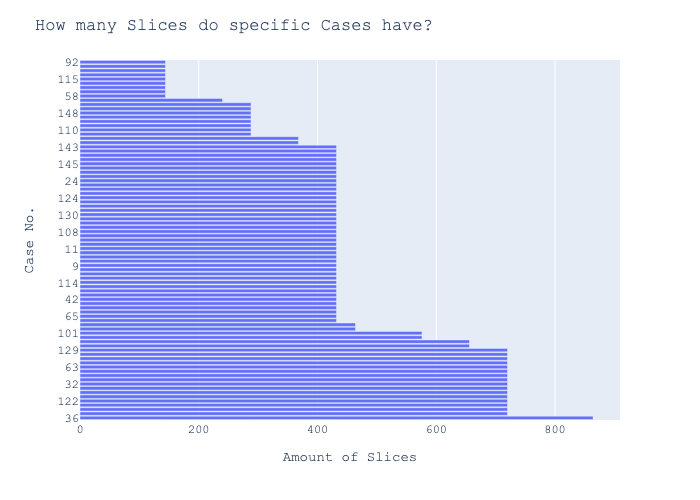
\includegraphics[width=1.2\linewidth]{bilder/slice_per_case}
     \caption{Anzahl Bilder pro Fall}\label{Fig:slice_per_case}
   \end{minipage}\hfill
   \begin{minipage}{0.48\textwidth}
     \centering
     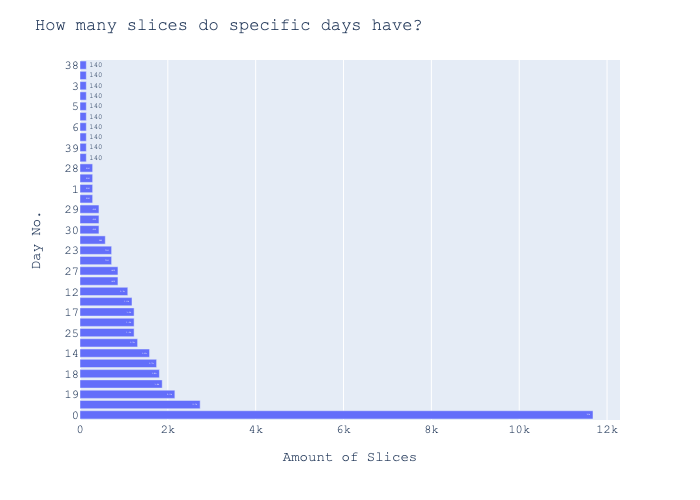
\includegraphics[width=1.2\linewidth]{bilder/slices_per_day}
     \caption{Anzahl Bilder pro Tag}\label{Fig:slice_per_day}
   \end{minipage}
\end{figure}

\subsection{Metadatenextraktion}




\subsection{Algorithmik}
?

\subsection{2.5 dimensionale Daten}
?

\subsection{Intelligentes Zuschneiden}
?

\subsection{Nachbearbeitung }
?

\subsection{Experimente}
Experimente.

\section{Evaluation}\raggedbottom

\section{Fazit}\raggedbottom

\subsection{Ausblick}
Ideen, die es nicht in die Arbeit geschafft haben oder nicht schafffen konnten.


\ifthenelse{\boolean{\biber}}{ % Beispiel um mit Biber zu zitieren (\citet und \citep)
	\citet{Con97} hat ein Buch geschrieben. Es gibt auch andere Arbeiten \citep{PeHe97} die referenziert sind. In Abbildung \ref{fig_Gallien} ist ein Sachverhalt dargestellt.


	1 Autor: \citet{Con97} \hspace*{1cm} \citep{Con97}\\
	2 Autoren: \citet{IWNLP} \hspace*{1cm} \citep{IWNLP}\\
	3 Autoren: \citet{liebeck-esau-conrad:2016:ArgMining2016} \hspace*{1cm} \citep{liebeck-esau-conrad:2016:ArgMining2016}

	Online resource: \citet{ILSVRC2016}
}{ %  Beispiel um klassisch zu zitieren (\cite)
	\cite{Con97} hat ein Buch geschrieben. Es gibt auch andere Arbeiten \cite{PeHe97} die referenziert sind. In Abbildung \ref{fig_Gallien} ist ein Sachverhalt dargestellt.


	1 Autor: \cite{Con97} \hspace*{1cm} \cite{Con97}\\
	2 Autoren: \cite{IWNLP} \hspace*{1cm} \cite{IWNLP}\\
	3 Autoren: \cite{liebeck-esau-conrad:2016:ArgMining2016} \hspace*{1cm} \cite{liebeck-esau-conrad:2016:ArgMining2016}

	Online resource: \cite{ILSVRC2016}
}

\ifthenelse{\equal{\sprache}{deutsch}}{
	\textbf{quotes}:\\
	Ein Beispiel für deutsche Anführungszeichen \glqq quote\grqq.
}{}

\begin{figure}[htb]
	\begin{center}
		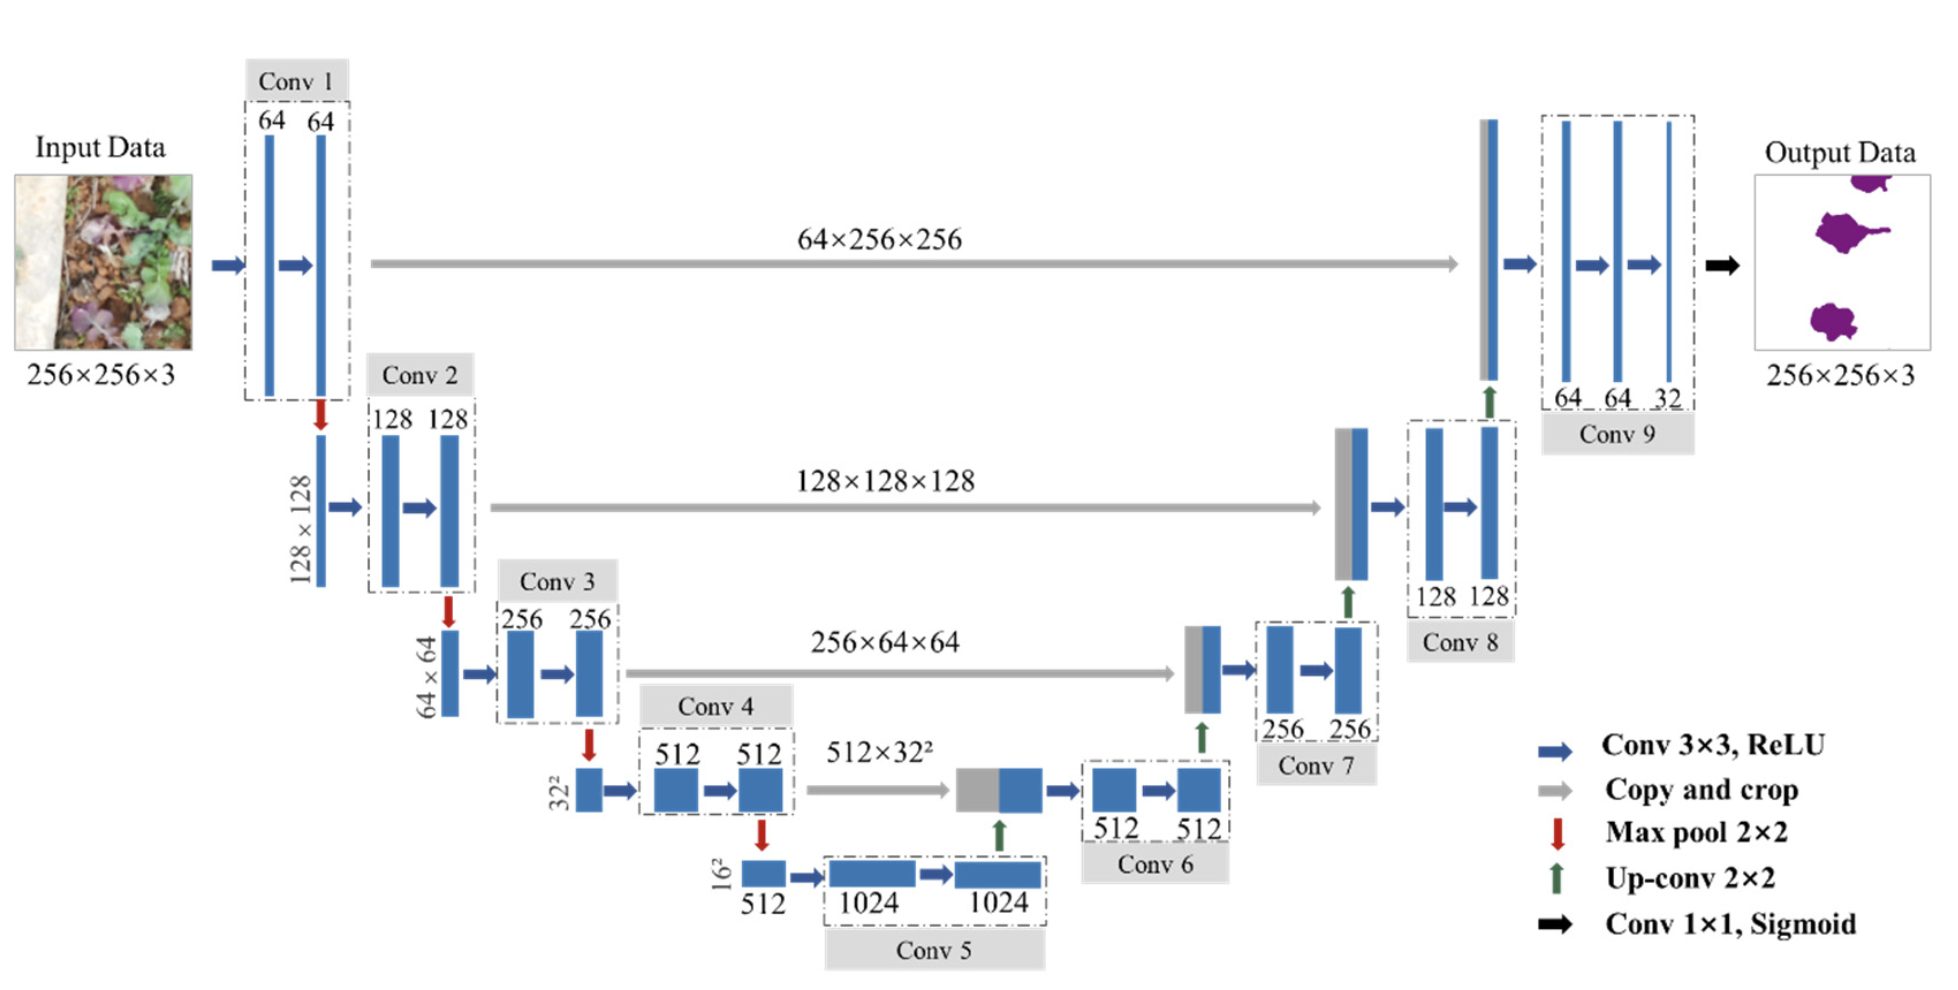
\includegraphics[width=300pt, angle=270]{bilder/u-net-architecture}
		\caption{U-Net Architektur}\label{Fig:unet-diagram}
	\end{center}
\end{figure}

\begin{figure}[htb]
	\begin{center}
		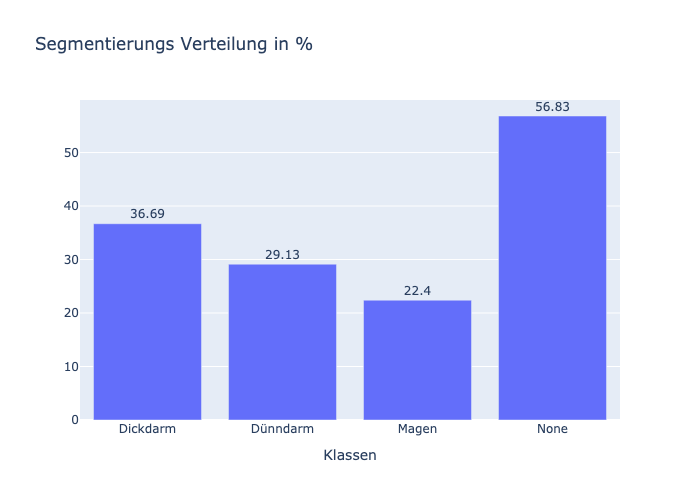
\includegraphics[width=220pt , angle=270]{bilder/segmentation_distribution}
		\caption{Verteilung der Klassen im Testset}\label{Fig:klassenverteilung}
	\end{center}
\end{figure}

\begin{figure}[htb]
	\begin{center}
		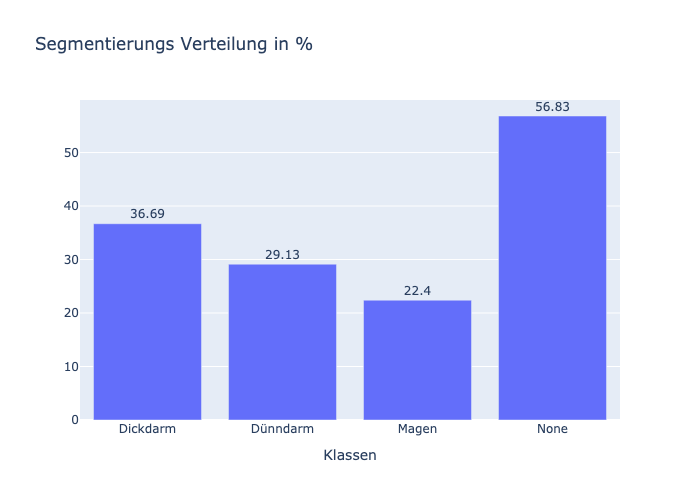
\includegraphics[width=220pt , angle=270]{bilder/segmentation_distribution}
		\caption{Verteilung der Klassen im Testset}\label{Fig:klassenverteilung}
	\end{center}
\end{figure}

\pagebreak

%%%%%%%%%%%%%%%%%%%%%%%%%%%%%%%%%%%%%%%%%%%%%%%%%%%%%%%%%%%%%%%%%%%%%%%%
%%%% ENDE TEXTTEIL %%%%%%%%%%%%%%%%%%%%%%%%%%%%%%%%%%%%%%%%%%%%%%%%%%%%%
%%%%%%%%%%%%%%%%%%%%%%%%%%%%%%%%%%%%%%%%%%%%%%%%%%%%%%%%%%%%%%%%%%%%%%%%

\clearpage

% Entfernen Sie das Kommentar aus der nachfolgenden Zeile, falls Sie einen Anhang in der Arbeit verwenden wollen. Beachten Sie, dass Sie sich im Verlauf der Arbeit mit \ref{...} (z.B. \ref{anhang:zusatz1}) auf den Anhang beziehen.
%\newpage
\appendix
\section{Anhang}

\subsection*{Zusatzteil 1} \label{anhang:zusatz1}

Dies ist ein Anhang.

\clearpage

\ifthenelse{\boolean{\biber}}{ %with biber do
	\DeclareNameAlias{sortname}{first-last}
	\printbibliography[heading=bibintoc, title=\references]
}{ %without biber do
	\bibliography{references}
	\bibliographystyle{alphadin}
}
%\vspace*{\fill}

\clearpage

\listoffigures

\listoftables

%\pagebreak

%\printindex
\end{document}
